\section{Simulations}

\subsection{Numerical implementation}

\subsubsection{Evolution equation}

Starting from \autoref{eq:eq1}, we want to obtain an equation to numerically calculate the wave height at the next timestep \(t_{i+1}\) using the previous heights at positions \(x_i\), \(x_{i-1}\) and \(x_{i+1}\). Using the following approximations for the derivatives
\begin{equation}
    \frac{\partial F}{\partial x}(x_i) \approx \frac{F(x_{i+1}) - F(x_{i-1})}{2 \Delta x}
    , \qquad
    \frac{\partial^2 F}{\partial x^2}(x_i) \approx \frac{F(x_{i+1}) - 2 F(x_i) + F(x_{i-1})}{(\Delta x)^2}
\end{equation}
where \(F\) is a generic function representing either \(f\) or \(h_0\), \(\Delta x = x_{i+1} - x_i\) as the mesh is regular and \(x\) is a generic variable representing either \(x\) or \(t\). \autoref{eq:eq1} is equivalent to:
\begin{equation}
    \frac{\partial^2 f}{\partial t^2} = g \frac{\partial h_0}{\partial x} \frac{\partial f}{\partial x} + g h_0 \frac{\partial^2 f}{\partial x^2}
\end{equation}
Then using the previously mentioned formulas:
\begin{equation}
    \begin{aligned}
        \frac{f(x_i, t_{i+1}) - 2 f(x_i, t_i) + f(x_i, t_{i-1})}{(\Delta t)^2} &= g \left( \frac{h_0(x_{i+1}) - h_0(x_{i-1})}{2 \Delta x} \right) \left( \frac{f(x_{i+1}, t_i) - f(x_{i-1}, t_i)}{2 \Delta x} \right) \\
        &+ g h_0(x_i) \frac{f(x_{i+1}, t_i) - 2 f(x_i, t_i) + f(x_{i-1}, t_i)}{(\Delta x)^2}
    \end{aligned}
\end{equation}
By rearanging and identifying the Courant-Friedrichs-Lewy constant \(\beta(x) = u(x) \frac{\Delta t}{\Delta x} = \sqrt{g h_0(x)} \frac{\Delta t}{\Delta x}\) we get the following equation:
\begin{equation}
    \begin{aligned}
        f(x_i, t_{i+1}) &= \frac{1}{4} \left( \beta(x_{i+1})^2 - \beta(x_{i-1})^2 \right) \left( f(x_{i+1}, t_i) - f(x_{i-1}, t_i) \right) \\
        &+ \beta(x_i)^2 (f(x_{i+1}, t_i) - 2 f(x_i, t_i) + f(x_{i-1}, t_i)) \\
        &+ 2 f(x_i,t_i) \\
        &- f(x_i,t_{i-1})
    \end{aligned}
\end{equation}
The evolution for \autoref{eq:eq2} is taken from \cite{physnumbook}, equation 4.43.

\subsubsection{Border conditions}

The simulation implements border conditions for a fixed border (the wave has a specific height at the border), a free border (the wave is allowed to move as it pleases along the border) and an exit condition (the wave continues as if there was no border). These conditions are given in the numerical physics book \cite{physnumbook} (section 4.2.1), for the left and right borders for exit and free borders as well as the exit condition for the right border. We will derive the exit conditions for the left border here. Under this condition, the left border only has a retrograde wave, i.e. \(f(x, t) = f_+(x + u t)\). Differentiating w.r.t. to \(t\) and \(x\), at \(x = x_L\) (left border) we obtain the following relationship:
\begin{gather}
    \frac{\partial f}{\partial t}(x_L, t) = \frac{\partial f_+(x_L + u t)}{\partial t} = u f_+'(x_L + u t) \\
    \frac{\partial f}{\partial x}(x_L, t) = f_+'(x_L + u t) \\
    \implies \frac{\partial f}{\partial t}(x_L, t) = u \frac{\partial f}{\partial x}(x_L, t)
\end{gather}
Discretising using the "forward" finite difference method, i.e. \(\frac{\partial F(x_i)}{\partial x} \approx (F(x_{i+1}) - F(x_i))/\Delta x\), for both time and space derivatives, and identifying \(x_L \equiv x_0\) the first position in the discretised list, we get:
\begin{equation}
    \frac{f(x_0,t_{n+1}) - f(x_0, t_n)}{\Delta t} = u \frac{f(x_1, t_n) - f(x_0, t_n)}{\Delta x}
\end{equation}
Rearanging and identifying the CFL constant we then get:
\begin{equation}
    f(x_0, t_{n+1}) = f(x_0, t_n) + \beta \left( f(x_1, t_n) - f(x_0, t_n) \right)
\end{equation}

\subsubsection{Initial conditions}

The initial conditions for a left and right moving wave, as well as a static wave were implemented using equations 4.48 to 4.50 given in \cite{physnumbook}.

The initial position and height of the wave can also be chosen to be either:
\begin{equation}
    f_\textrm{init}(x) = \begin{cases}
        \begin{aligned}
            &0 &&(x \le x_1)\\
            & {\frac{A}{2} \left( 1 - \cos \left( 2\pi\frac{x-x_1}{x_2-x_1} \right) \right)} &&(x_1 < x < x_2)\\
            &0 &&(x_2 \le x)
        \end{aligned}
    \end{cases}
\end{equation}
or initialised in normal modes according to \autoref{eq:normal_initial}.




\subsection{Wave with constant velocity}
In this first simulation we consider a basin going from $x_L = 0$ \si{\meter} to $x_R = 10$ \si{\meter}. The water inside of it has a constant depth of $h_0(x) = 3$ \si{\meter} $\, \forall x$













\subsection{Oceanic wave on a coral reef}

In this section we will use the following function for oceanic depth:
\begin{equation}
    h_0(x) = \begin{cases}
        \begin{aligned}
            &h_L &&(x_L \le x \le x_a) \\
            &\frac{1}{2}(h_L + h_C) + \frac{1}{2}(h_L - h_C) \cos \left( \pi \frac{x-x_a}{x_b-x_a} \right) &&(x_a < x < x_b) \\
            &h_C &&(x_b \le x \le x_c) \\
            &\frac{1}{2}(h_R + h_C) - \frac{1}{2}(h_R - h_C) \cos \left( \pi \frac{x-x_c}{x_d-x_c} \right) &&(x_c < x < x_d) \\
            &h_R &&(x_d \le x \le x_R)
        \end{aligned}
    \end{cases}
\end{equation}
We will choose \(h_L = 7000\)m, \(h_C = 35\)m, \(h_R = 200\)m, \(x_L = 0\)m, \(x_a = 300\)km, \(x_b = 700\)km, \(x_c = 720\)km, \(x_d = 850\)km and \(x_R = 1000\)km. The initial conditions will be a right moving wave with \(x_1 = 50\)km, \(x_2 = 250\)km and amplitude \(A = 1\)m. Both border conditions will be set to exit, to be more representative of an actual large ocean. The simulations were done until the wave passes the coral reef entierely, which corresponds to a time of about \(t = 12000\). The timestep \(\Delta t\) was chosen such that \(\max(\beta_{\textrm{CFL}}) = 1\), which is \(\Delta t = \Delta x / \max_x(u(x)^2)\). The number of intervals was chosen to be 8192.

\autoref{fig:corail_eq1_mouv} shows the obtained wave motion when using \autoref{eq:eq1}. The depth profile is shown in \autoref{fig:corail_eq1_depth}. We can see that around \(x=600\)km, the wave slows down considerably with a peak in amplitude, which corresponds to when the wave is right above the reef. We will study the amplitude and speed later. The observed behavior makes sense intuitively, as a wave would indeed get larger when the water becomes less deep.

\begin{figure}[h]
    \centering
    \begin{subfigure}{0.53\linewidth}
        \centering
        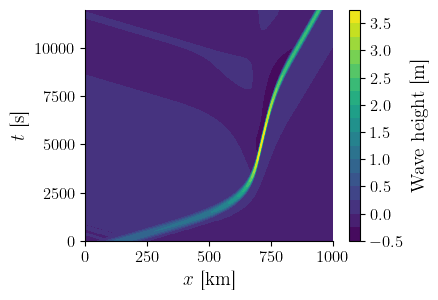
\includegraphics[width=\linewidth]{figures/corail_eq1_mouvement_vague.png}
        \caption{Wave function}
        \label{fig:corail_eq1_mouv}
    \end{subfigure}
    \begin{subfigure}{0.46\linewidth}
        \centering
        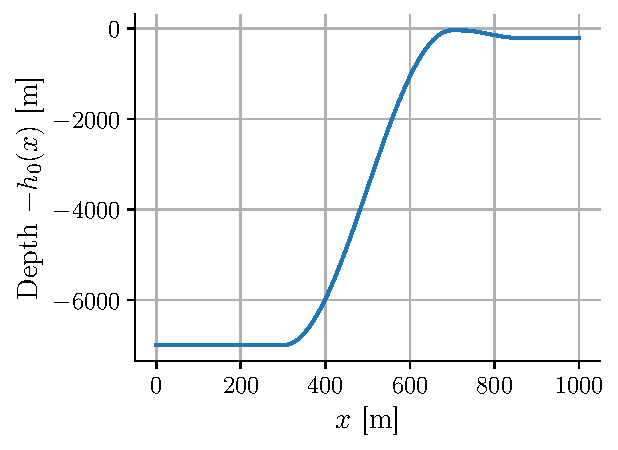
\includegraphics[width=\linewidth]{figures/corail_eq1_depth.pdf}
        \caption{Depth profile}
        \label{fig:corail_eq1_depth}
    \end{subfigure}
    \caption{Wave height as a function of space and time and depth profile. Simulated using \(n=8192\) intervals, until \(t=12000\)}
\end{figure}

The maximum amplitude of the wave was obtained using a quadratic fit for every point around the time of its maximum amplitude. The maximum of the fit gave the maximum amplitude. Results are shown in \autoref{fig:corail_eq1_amplitude}. The simulation shows that the maximum amplitude increase up to the point of the coral reef, remains more or less constant on top of the reef and then goes back down. The peak amplitude above the reef (\(x_b < x < x_c\)) was found to be about 3.58m, while after the reef (\(x_d<x<x_R\)) the maximum amplitude was 2.30m. When compared to the WKB solution of \autoref{eq:eq1} given in \cite{physnumbook}, we notice that the amplitude is a bit lower than expected on top and after the reef, while it matches almost exactly before the reef. This discrepency can be attributed to either numerical imprecision or the effect of higher order terms.

Using the analysis done on the amplitude, the speed of the peak of the wave was calculated using the time \(t_{\textrm{peak},i}\) at which the fitted function is maximal. Then for every point \(x_i\), except for border cases, the speed is given by \(v_i = (x_{i+k} - x_{i-k})/(t_{\textrm{peak},i+k} - t_{\textrm{peak},i-k})\), where \(k\) is chosen such that the oscillations in \(v\) are minimal. The results are shown in \autoref{fig:corail_eq1_vitesse}. We can see that the speed decrease drastically between the starting position of the wave and the coral reef, by a factor of about 11: the speed above the reef was found to be 18 m/s, while the initial speed was 261 m/s. After the reef, the speed increases again to around 42 m/s. The simulation matches the WKB solution exactly.

\begin{figure}[h]
    \centering
    \begin{subfigure}{0.48\linewidth}
        \centering
        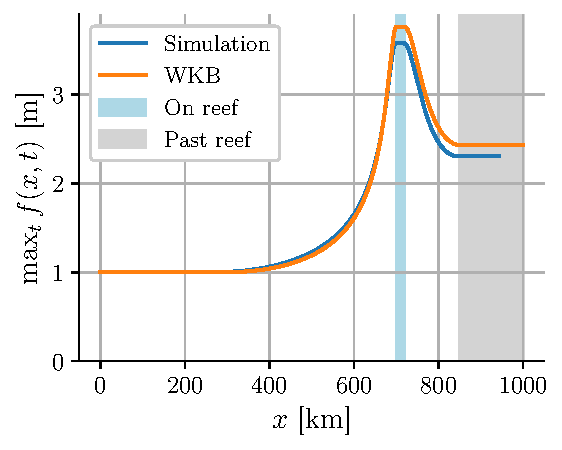
\includegraphics[width=\linewidth]{figures/corail_eq1_amplitude_wkb.pdf}
        \caption{Maximum amplitude reached at each position}
        \label{fig:corail_eq1_amplitude}
    \end{subfigure}
    \begin{subfigure}{0.48\linewidth}
        \centering
        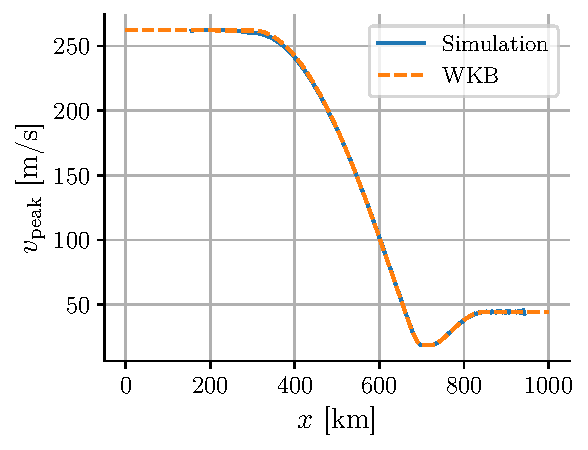
\includegraphics[width=\linewidth]{figures/corail_eq1_vitesse_wkb.pdf}
        \caption{Speed of wave peak}
        \label{fig:corail_eq1_vitesse}
    \end{subfigure}
    \caption{Properties of the wave going towards the coral reef, compared to WKB solution. Simulated using \(n=8192\) intervals, until \(t=12000\)}
    \label{fig:corail_eq1_properties}
\end{figure}

We would now like to analyse what happens when the slope becomes really steep, by setting \(x_a\) closer and closer to \(x_b\). Here we chose to look at case where the distance between \(x_b\) and \(x_a\) was 100km and 50km, as the 400km case was treated previously. \autoref{fig:corail_eq1_mouv_xa=60km} and \autoref{fig:corail_eq1_mouv_xa=65km} show the obtained wave function. The depth profile for both cases is also shown in \autoref{fig:corail_eq1_depth_xa}. We notice an interesting phenomenon: as the slope becomes steeper, a large part of the wave gets reflected at the reef. This is similar to a change in medium, with different density, leading to a greater reflected wave and a smaller transmitted one.

\begin{figure}[h]
    \centering
    \begin{subfigure}{0.48\linewidth}
        \centering
        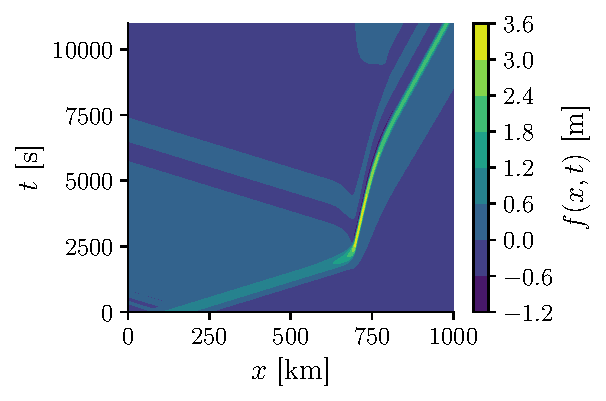
\includegraphics[width=\linewidth]{figures/corail_eq1_movement_xa=600000.pdf}
        \caption{\(x_a = 60\)km}
        \label{fig:corail_eq1_mouv_xa=60km}
    \end{subfigure}
    \begin{subfigure}{0.48\linewidth}
        \centering
        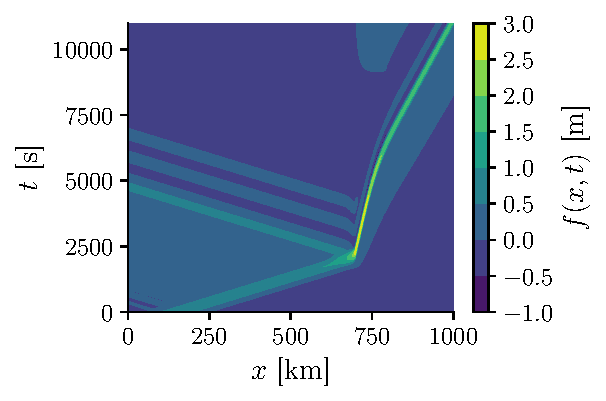
\includegraphics[width=\linewidth]{figures/corail_eq1_movement_xa=650000.pdf}
        \caption{\(x_a = 65\)km}
        \label{fig:corail_eq1_mouv_xa=65km}
    \end{subfigure}
    \caption{Wave height as a function of space and time. Simulated using \(n=8192\) intervals until \(t=12000\)}
    \label{fig:corail_eq1_mouv_xa}
\end{figure}

\begin{figure}[h]
    \centering
    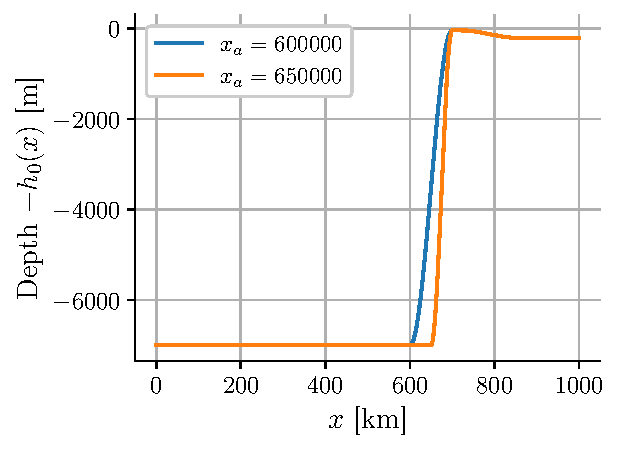
\includegraphics[width=0.6\linewidth]{figures/corail_eq1_depth_var_xa.pdf}
    \caption{Depth profile for different \(x_a\)}
    \label{fig:corail_eq1_depth_xa}
\end{figure}

Using the same analysis methods as before, we obtain the amplitude in \autoref{fig:corail_eq1_amplitude_xa=60km} and \autoref{fig:corail_eq1_amplitude_xa=65km}. We notice that as the slope gets steeper, the simulated wave becomes less and less high when on the reef. Compared to the WKB solution, the simulation severely undershoots, with a difference of about 1m on and after the reef for \(x_a = 65\)km. This difference can be attributed by the fact that WKB suppose a reasonably small change in depth, while this change of about 7000m over 50km could be considered "too fast". For the speed of the wave, the \autoref{fig:corail_eq1_speed_xa=60km} and \autoref{fig:corail_eq1_speed_xa=65km}, we notice that the simulations follows the WKB solution closely, except when near the cliff, with the effect being more important for \(x_a = 65\)km. This effect does not seem physical and could be attributed to numerical effects: if we consider a vertical slope, the wave would travel across an interface between to "mediums" with different propagation speeds, the speed would only change rapidly at the interface and not before.

\begin{figure}[h]
    \centering
    \begin{subfigure}{0.48\linewidth}
        \centering
        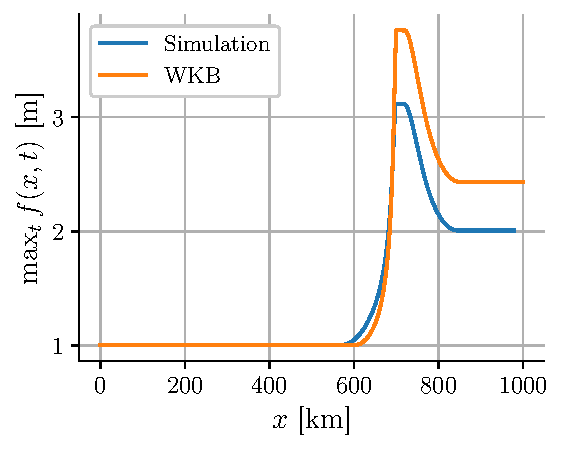
\includegraphics[width=\linewidth]{figures/corail_eq1_amplitude_xa=600000.0.pdf}
        \caption{Maximum amplitude}
        \label{fig:corail_eq1_amplitude_xa=60km}
    \end{subfigure}
    \begin{subfigure}{0.48\linewidth}
        \centering
        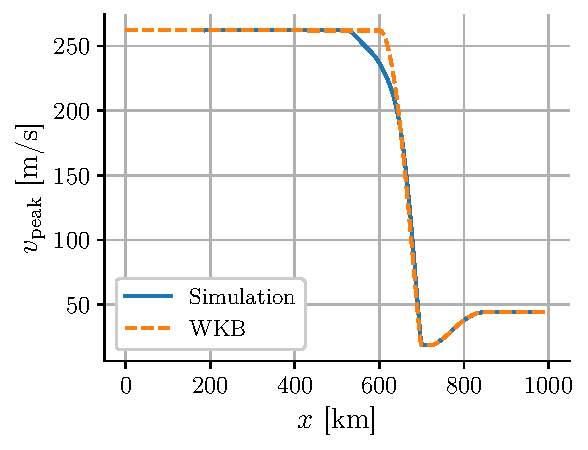
\includegraphics[width=\linewidth]{figures/corail_eq1_vitesse_xa=600000.0.pdf}
        \caption{\(x_a = 65\)km}
        \label{fig:corail_eq1_speed_xa=60km}
    \end{subfigure}
    \caption{Wave properties for \(x_a = 60\)km. Simulated using \(n=8192\) intervals until \(t=12000\)}
\end{figure}

\begin{figure}[h]
    \centering
    \begin{subfigure}{0.48\linewidth}
        \centering
        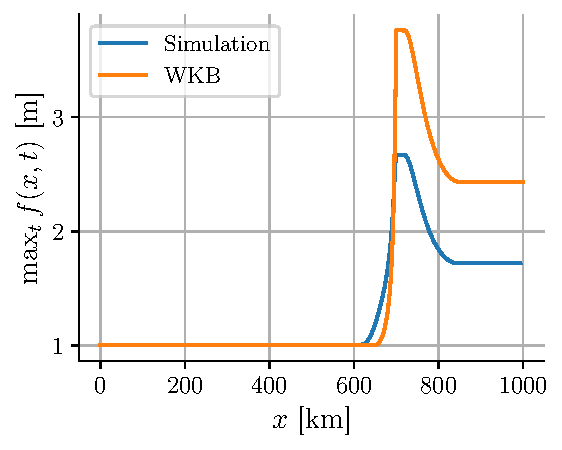
\includegraphics[width=\linewidth]{figures/corail_eq1_amplitude_xa=650000.0.pdf}
        \caption{Maximum amplitude}
        \label{fig:corail_eq1_amplitude_xa=65km}
    \end{subfigure}
    \begin{subfigure}{0.48\linewidth}
        \centering
        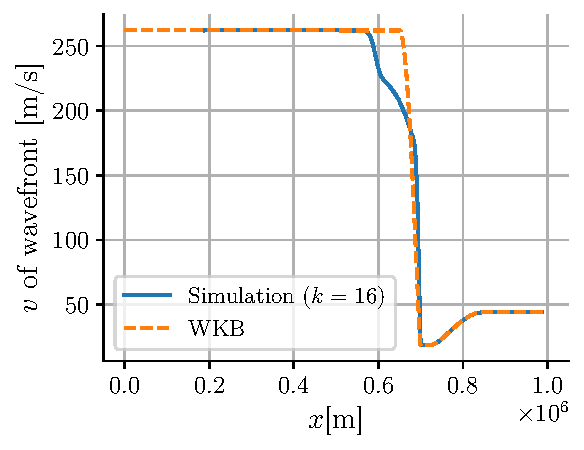
\includegraphics[width=\linewidth]{figures/corail_eq1_vitesse_xa=650000.0.pdf}
        \caption{\(x_a = 65\)km}
        \label{fig:corail_eq1_speed_xa=65km}
    \end{subfigure}
    \caption{Wave properties for \(x_a = 65\)km. Simulated using \(n=8192\) intervals until \(t=12000\)}
\end{figure}


Let's now analyse what happens when we simulate the system using the wrong although maybe intuitively plausible equation, \autoref{eq:eq2}. The resulting wave can be seen in \autoref{fig:corail_eq2_mouvement}. While the result looks similar at a glance to the result at the begining of this section, we can see that the amplitude of the wave decreases above the reef! Analysing this further using the same methods as described previously, we obtain a plot of the maximal amplitude and speed of the wave peak shown in \autoref{fig:corail_eq2_amplitude}. This time, the simulation undershoots the WKB solution, starting from where the depth changes. The difference between the simulation and the WKB solution remains under 0.02m, which is still quite precise. Like previously howether, the speed matches the WKB solution exactly, as can be seen in \autoref{fig:corail_eq2_vitesse}. The WKB analysis on both equations showed that the speed is the same for both equations, which was verified again here.

\begin{figure}[h]
    \centering
    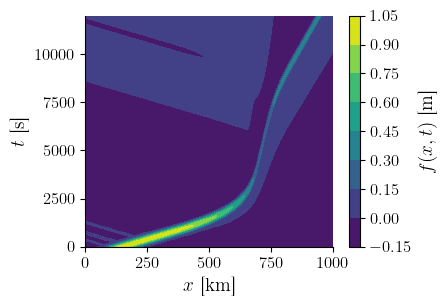
\includegraphics[width=0.6\linewidth]{figures/corail_eq2_mouvement_vague.png}
    \caption{Wave height as a function of space and time, simulated following \autoref{eq:eq2}. Simulated with \(n=16328\) intervals until \(t=12000\)}
    \label{fig:corail_eq2_mouvement}
\end{figure}

\begin{figure}[h]
    \centering
    \begin{subfigure}{0.48\linewidth}
        \centering
        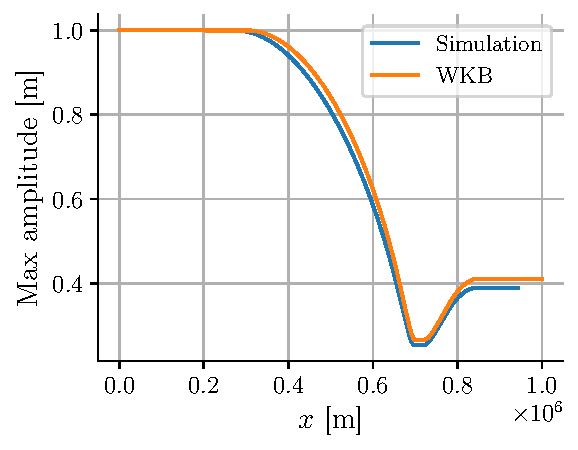
\includegraphics[width=\linewidth]{figures/corail_eq2_amplitude_wkb.pdf}
        \caption{Maximum amplitude reached at each position}
        \label{fig:corail_eq2_amplitude}
    \end{subfigure}
    \begin{subfigure}{0.48\linewidth}
        \centering
        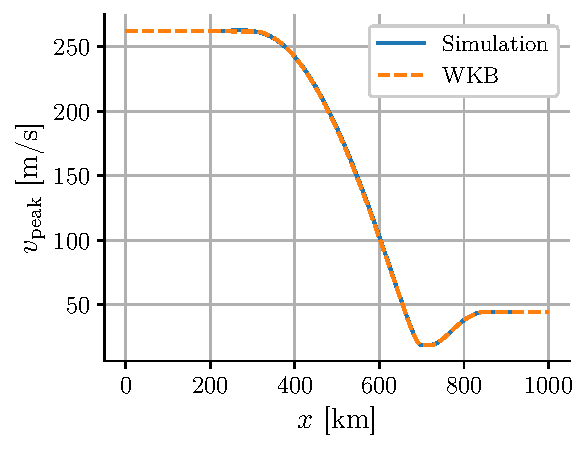
\includegraphics[width=\linewidth]{figures/corail_eq2_vitesse_wkb.pdf}
        \caption{Speed of wave peak}
        \label{fig:corail_eq2_vitesse}
    \end{subfigure}
    \caption{Properties of the wave going towards the coral reef, compared to WKB solution. Simulated w.r.t. \autoref{eq:eq2}, using \(n=8192\) intervals, until \(t=12000\)}
    \label{fig:corail_eq2_properties}
\end{figure}